\documentclass[11pt]{model1}

% packages
\usepackage[dvips]{graphicx}
\usepackage[french]{babel}
\addto\captionsfrench{\renewcommand{\chaptername}{Section}}
\usepackage[T1]{fontenc}
\usepackage{amsmath,amssymb,bbm} % math, mathbb, mathbbm

\usepackage{url} %% pour citer les url par \url
\usepackage{natbib} %% pour plus de flexibilité dans les citations
\usepackage{makeidx} %% index
\usepackage{rotating} %% pour rotate
\usepackage{multirow} %% pour regrouper un texte sur plusieurs lignes dans une table\usepackage{multirow}
\usepackage{color} 

%\usepackage{moreverb} %% pour le verbatim en boite
%\usepackage{slashbox} %% pour couper les colonnes des tableaux en diagonale 
%\usepackage{showkeys} %% pour voir les labels
%\usepackage[all]{xy} %% pour la barre au dessus des symboles
%\usepackage{shorttoc} %% pour plusieurs tables des matières par la commande \shorttableofcontents{Titre}{profondeur}.
%\usepackage{textcomp} %% pour le symbol pour mille par \textperthousand.
%\usepackage[dvips]{hyperref} % permet d'obtenir des liens sur les sections dans les PDF
%\usepackage[right]{eurosym}
%\usepackage{eurosans} %% pour le symbole \euro
%\usepackage{epic,eepic}
%\usepackage{times,palatino}  % fontes
%\usepackage{mathptm}
%\usepackage{comment} % pour cut

\headheight = 13.6pt

% macros, d�finitions et nouvelles commandes perso
\def\argmax{\operatornamewithlimits{arg\,max}}
\def\argmin{\operatornamewithlimits{arg\,min}}
\newcommand{\dtc}{\ensuremath{\operatorname{d_{tc}}}}

\DeclareMathOperator*{\Mult}{Mult}

 
\makeindex 
\graphicspath{{fig/}} 


\begin{document}
\thispagestyle{empty}
\begin{titlepage}
%\TitlePageDimension

\begin{sffamily}
\begin{bfseries}

\begin{empty}
 \vspace*{58mm}
\end{empty}

\begin{flushleft}
  \hspace{60mm}
  \noindent{\Large Reuven BENICHOU}
\end{flushleft}

\begin{flushleft}
  \hspace{60mm}
  \noindent{\Large Edern HOTTE}
\end{flushleft}

\begin{flushleft}
  \hspace{60mm}
  \noindent{\Large Flavien MOULLEC}
\end{flushleft}

\vspace*{6mm}

\hspace{55mm}
\begin{minipage}[c]{0mm}
  
\includegraphics[width=110mm]{font.eps}
\end{minipage}
  
\vspace*{5mm}

\begin{flushleft}
  \hspace{46mm}
  \noindent{\huge Optimisation de biblioth�que \hspace*{46mm} de calcul num�rique}
\end{flushleft}


  \hspace{55mm}
  \noindent{\large Rapport technique du projet 11 - version 2}

  \hspace{55mm}
  \noindent{\normalsize Date : 15 Juin 2011}



  \hspace{55mm}
  \noindent{\normalsize Encadrant : Serge GUELTON}
  \newline

  \hspace{55mm}
  \noindent{\normalsize Projet de d�veloppement - Semestre 2}



  \hspace{55mm}
  \noindent{\normalsize Ann�e scolaire 2010 - 2011}
  
  \hspace{55mm}
  \noindent{\small \`A destination du groupe de pilotage du projet S2}

\end{bfseries}
\end{sffamily}

\vspace*{11mm}
\hspace{60mm}
\begin{minipage}[c]{0mm}
  \includegraphics[width=28mm]{logo.eps}
\end{minipage}
%\ResetDefaultPageDimension
\end{titlepage}

\newpage
\thispagestyle{empty}
~

%\maketitle
\newpage\cleardoublepage

\markboth{}{}
%\pagestyle{empty}
%---------------------------%
\section*{R�sum�}

Ecrire le r�sum� ici

\section*{Abstract}

Ecrire la m�me chose en Anglais

\section*{Mot-cl�s}

5-6 max

\newpage\cleardoublepage\thispagestyle{empty}
\markboth{Table des matières}{Table des matières}
\tableofcontents

\chapter{Introduction}
\label{chap:introduction}

\section{Motivations }

Le projet 11 \citep{projet11}, intitul\'e << Optimisation de biblioth\`eque de calcul num\'erique >>, est un projet informatique bas\'e sur le langage C qui vise \`a am\'eliorer 
les performances de calcul de la biblioth\`eque num-utils \citep{numutils}, travaillant sur des flots de donn\'ees \citep{dataflux}.
Il aboutira au d\'eveloppement d'un vrai logiciel qui sera publi\'e dans les archives Debian \citep{debian}.

Ceci est \'evidemment une source de motivation non n\'egligeable. Mais \`a travers cet aspect concret de notre projet, c'est tout l'environnement d'un 
projet informatique, les contraintes impos\'ees , l'interface existante entre les d\'eveloppeurs, le travail d'optimisation, qui sont les raisons 
d'\^etre de ce travail.
Il s'inscrit alors dans un contexte pr\'ecis : le d\'eveloppement d'un projet informatique en vue de sa publication.

\section{Objectifs}

Bien que le projet repose sur une optimisation de performances, l'objectif principal reste la mise en place des outils n\'ecessaires en vue de la 
r\'ealisation et de la publication d'un logiciel dans les archives Debian.  

En effet derri\`ere la probl\'ematique d'optimisation se cache une autre probl\'ematique qui sera le point de d\'epart de notre projet : comment mettre
 en \oe{}uvre un projet informatique ? 
Notre d\'emarche consistera en premier lieu en la d\'ecouverte et l'utilisation des outils n\'ecessaires \`a la r\'ealisation d'un projet informatique afin 
de mettre en ligne une biblioth\`eque num-utils cod\'e en C.
\newline 	
Tout d'abord une impl\'ementation des algorithmes sera fournie en langage C avec l'ensemble des outils de d\'eveloppement mis en \oe{}uvre. Ensuite, 
un paquet Debian fournissant une distribution open source sera mise en ligne. 
Outre les d\'ecouvertes techniques, cette premi\`ere approche sera l'occasion de constater toute l'importance de la forme ( page de manuel, readme,...) 
lors de la conception d'un logiciel informatique publi\'e.

La seconde \'etape du projet sera l'optimisation des performances de calculs de nos codes C . Cette phase, plus courte, se veut diff\'erente de la 
premi\`ere : elle n\'ecessite avant tout un travail de r\'eflexion. C'est  un travail de fond o\`u l'objectif principal sera une division par 10 du temps
 d'ex\'ecution. 

Notre d\'emarche sera donc constitu\'ee de deux \'etapes : la mise en place d'un socle de travail, puis le travail de fond d'optimisation. Ces deux phases 
s'inscrivent dans le contexte du projet qui est le d\'eveloppement d'un projet informatique afin de r\'epondre \`a la probl\'ematique explicite du sujet 
qui est l'optimisation d'une biblioth\`eque de calcul num\'erique.


 % chapitre 1
\chapter{La biblioth\`eque num-utils}
\label{chap:La bibliotheque num-utils}

\section{Pr\'esentation}
\index{Perl}
\index{num-utils}
La biblioth\`eque de calcul num\'erique qu'il nous fallait am\'eliorer s'appelle num-utils. Elle est \'ecrite dans un langage
interpr\'et\'e, le Perl.
Le paquet num-utils est inclus dans la distribution officielle de Debian.

Elle impl\'emente un certain nombre d'algorithmes num\'eriques travaillant sur des flots de donn\'ees.
Ces algorithmes sont r\'epartis dans dix programmes diff\'erents s'intitulant : numaverage, numbound, numgrep, numinterval, numnormalize,
numprocess, numrandom, numrange, numround et numsum.

La premi\`ere am\'elioration que l'on pouvait apporter \`a la biblioth\`eque \'etait de passer d'un langage interpr\'et\'e en un langage compil\'e.
Nous avons ainsi cod\'e, en langage C, l'ensemble de ces utilitaires.

Nous avons respect\'e dans la mesure du possible les m\^emes notations et les m\^emes noms d'options que ceux de la biblioth\`eque num-utils.
Notre nouvelle biblioth\`eque s'appelle \textbf{num-utils-ng}.

\section{Fonctionnalit\'es propos\'ees par ces dix programmes}

\subsection{Points communs de chaque utilitaire}
Cette partie explique en d\'etail les fonctionnalit\'es propos\'es par ces diff\'erents programmes.
Les dix programmes constituant la biblioth\`eque num-utils-ng s'ex\'ecutent en ligne de commande dans un terminal Unix (shell).
Pour chacun de ces programmes, except\'e numrandom qui ne prend aucune donn\'ee en entr\'ee, les donn\'ees sont lues \`a partir 
de l'entr\'ee standard (stdin) ou \`a partir d'un fichier.
Ces dix programmes proposent chacun une option << \textbf{-h} >> permettant \`a l'utilisateur d'obtenir une aide sur le fonctionnement du 
programme sous la forme d'une page de manuel (man pages en anglais).

\subsection{Calculs simples sur des nombres d\'ecimaux}

Cette partie regroupe trois programmes : numaverage, numnormalize et numsum.
\newline
\begin{itemize}\index{numaverage}
 \item[\textbullet] \textbf{numaverage :} numaverage retourne la moyenne des nombres relatifs pass\'es en entr\'ee.
Ce programme propose cinq options :
\begin{itemize}
  \item[-] << \textbf{-i} >> : retourne la partie enti\`ere de la moyenne,
  \item[-] << \textbf{-I} >> : retourne la partie d\'ecimale de la moyenne,
  \item[-] << \textbf{-m} >> : retourne le nombre qui appara\^it le plus souvent,
  \item[-] << \textbf{-M} >> : retourne le nombre m\'edian,
  \item[-] << \textbf{-l} >> : retourne le nombre m\'edian le plus petit (utile quand le nombre total d\'el\'ements est pair).
\newline
\end{itemize}\index{numnormalize}
\item[\textbullet] \textbf{numnormalize :} numnormalize prend un ensemble de nombres en entr\'ee et retourne l'ensemble de ces nombres, 
normalis\'es entre 0 et 1 par d\'efaut. Il propose une seule option :
\begin{itemize}
 \item[-] << \textbf{-R <n1>..<n2>} >> : la normalisation est effectu\'ee entre les nombres <n1> et <n2>.
\newline
\end{itemize}\index{numsum}
 \item[\textbullet] \textbf{numsum :} numsum retourne la somme des nombres relatifs pass\'es en entr\'ee.
Six options sont propos\'ees :
\begin{itemize}
 \item[-] << \textbf{-i} >> : retourne la partie enti\`ere de la somme,
 \item[-] << \textbf{-I} >> : retourne la partie d\'ecimale de la somme,
 \item[-] << \textbf{-c} >> : retourne la somme de chaque colomne,
 \item[-] << \textbf{-r} >> : retourne la somme de chaque ligne,
 \item[-] << \textbf{-x <n>} >> : retourne la somme des colomnes d\'efinies dans l'ensemble <n>,
 \item[-] << \textbf{-y <n>} >> : retourne la somme des lignes d\'efinies dans l'ensemble <n>.
\end{itemize}
\end{itemize}

\subsection{Comparaisons de nombres d\'ecimaux}

Cette partie regroupe trois programmes : numbound, numinterval et numround.
\newline
\begin{itemize}\index{numbound}
 \item[\textbullet]  \textbf{numbound :} numbound renvoie le plus grand nombre pass\'e en entr\'ee.
Ce programme propose une seule option :
\begin{itemize}
  \item << \textbf{-l} >> : retourne le plus petit nombre pass\'e en entr\'ee.
\newline
\end{itemize}\index{numinterval}
 \item[\textbullet] \textbf{numinterval :} numinterval calcule et affiche l'intervalle entre un nombre et le suivant du flux d'entr\'ee.
Ce programme ne poss\`ede pas d'options sp\'ecifiques.
\newline\index{numround}
 \item[\textbullet] \textbf{numround :} numround arrondit le nombre d\'ecimal pass\'e en entr\'e en l'entier le plus proche.
Ce programme propose trois options :
\begin{itemize}
 \item[-] << \textbf{-c} >> : renvoie la partie enti`ere du nombre en entr\'ee,
 \item[-] << \textbf{-f} >> : renvoie l'entier imm\'ediatement sup\'erieur \`a la valeur du nombre en entr\'ee, 
 \item[-] << \textbf{-n <n>} >> : renvoie le multiple de l'entier <n> le plus proche du nombre en entr\'ee.
\end{itemize}
\end{itemize}

\subsection{G\'en\'eration et modifications de nombre d\'ecimaux}

Cette partie regroupe quatre programmes : numgrep, numprocess, numrandom et numrange.
\newline
\begin{itemize}\index{numgrep}
 \item[\textbullet] \textbf{numgrep :} numgrep retourne l'ensemble des nombres v\'erifiant la condition pass\'ee en argument. La condition est de la
forme << /expression/ >>. Les diff\'erentes expressions possibles sont les suivantes :
  \begin{itemize}
  \item[-] << \textbf{/<n1>..<n2>/} >> : retourne l'ensemble des nombres appartenant \`a l'intervalle [n1,n2], n1 et n2 \'etant des entiers.
  \item[-] << \textbf{/m<n>/} >> : retourne l'ensemble des multiples du nombre <n>,
  \item[-] << \textbf{/f<n>/} >> : retourne l'ensemble des diviseurs du nombre <n>.
  \end{itemize}
Remarque : Ces expressions peuvent \^etre combin\'ees en les s\'eparant par une virgule << \textbf{,} >>.
\newline\index{numprocess}
 \item[\textbullet] \textbf{numprocess :} numprocess effectue une liste d'op\'erations sur l'ensemble des nombres pass\'es en entr\'ee.
Les op\'erations possibles sont d\'ecrite dans le tableau 2.1 ci-dessous. Deux constantes sont \'egalement d\'efinies : << \textbf{pi} >> 
et << \textbf{e} >>, repr\'esentant respectivement $\Pi$ et $e^1$.
\begin{table}[h]
\begin{center}

\begin{tabular}{|l|c|r|}
  \hline
  Symbole &  Op\'eration\\
  \hline
  << \textbf{+} >> & Addition \\
  << \textbf{-} >> & Soustraction \\
  << \textbf{*} >> & Multiplication \\
  << \textbf{\%} >> & Division \\
  << \textbf{\^} >> & Puissance \\
  << \textbf{sqrt} >> & Racine carr\'ee \\
  << \textbf{sin} >> & Sinus \\
  << \textbf{cos} >> & Cosinus \\
  \hline
\end{tabular}
\caption{Symboles utilis\'es dans numprocess}
\end{center}
\label{tab:symboles}
\end{table}
\newline\index{numrandom}
 \item[\textbullet] \textbf{numrandom :} numrandom retourne un nombre g\'en\'er\'e al\'eatoirement. Par d\'efaut, ce nombre est un entier entre 1 et 100.
Le programme peut prendre un argument de la forme << /expression/ >>. Les diff\'erentes expressions possibles sont les suivantes :
\begin{itemize}
 \item[-] << \textbf{/<n1>:<n2>/} >> : retourne un entier  g\'en\'er\'e al\'eatoirement entre les nombres <n1> et <n2>, avec un pas de 1,
 \item[-] << \textbf{/<n1>:<n2>i<p>/} >> : retourne un entier  g\'en\'er\'e al\'eatoirement entre <n1> et <n2>, avec un pas <p>.
\end{itemize}
Remarque : Ces expressions peuvent \^etre combin\'ees en les s\'eparant par une virgule << \textbf{,} >>.
\newline\index{numrange}
 \item[\textbullet] \textbf{numrange :} numrange affiche la liste des nombre v\'erifiant la condition pass\'ee en argument de la forme << /expression/ >>.
Les diff\'erentes expressions possibles sont les suivantes :
\begin{itemize}
 \item[-] << \textbf{/<n1>:<n2>/} >> : retourne la liste des nombres compris entre <n1> et <n2>, avec un pas de 1,
 \item[-] << \textbf{/<n1>:<n2>i<p>/} >> : retourne la liste des nombres compris entre <n1> et <n2>, avec un pas <p>. 
\end{itemize}
Trois options sont \'egalement propos\'ees :
\begin{itemize}
 \item[-] << \textbf{-e <e>} >> : exclut la liste des nombres se trouvant dans l'ensemble <e>,
 \item[-] << \textbf{-n <s>} >> : chaque nombre du flux d'entr\'ee est s\'epar\'e par le caract\`ere <s>. Par d\'efaut, le s\'eparateur est l'espace.
 \item[-] << \textbf{-N} >> : chaque nombre du flux d'entr\'ee est s\'epar\'e par le caract\`ere de retour \`a la ligne.
\end{itemize}
\end{itemize}

\section{Utilit\'e de ces programmes}

Les dix programmes pr\'esent\'es ci-dessus sont relativement simple \`a utiliser. Chacun ne pr\'esente qu'une fonction principale ainsi que quelques options.
Ce type de programme est donc appr\'eci\'e des programmeurs, par sa facilt\'e et sa rapidit\'e d'ex\'ecution. Dans le chapitre \ref{chap:tests et optimisations}
nous pr\'esenterons en d\'etail les performances obtenues.
\newline
Exemples d'utilisation de ces programmes :
\begin{itemize}
 \item[-] \'Ecrire dans result.txt l'ensemble des multiples de 12 contenus data.txt :
 \begin{verbatim} numgrep /m12/ data.txt >result.txt \end{verbatim}
 \item[-] Normaliser (entre 0 et 1) les nombres contenus dans data.txt:
 \begin{verbatim} numnormalize data.txt \end{verbatim}
 \item[-] G\'en\'erer un ensemble d'\'echantillons dans l'intervalle [1,100] avec un pas de 0.2 :
 \begin{verbatim} numrange /1:100:0.2/ \end{verbatim}
 \item[-] En choisir un al\'eatoirement :
 \begin{verbatim} numrandom /1:100:0.2/ \end{verbatim}
\end{itemize}

Ces exemples ne sont que quelques cas d'utilisations des fonctions de la biblioth`eque num-utils-ng que nous avons optimis\'e.


 % chapitre 2
\chapter{Outils utilis\'es}
\label{chap:outils utilises}

\section{Section }
 % chapitre 3	

\chapter{Tests et optimisations}
\label{chap:tests et optimisations}

\section{Pr\'esentation}

Apr\`es avoir pr\'esent\'e les outils que nous avons utilis\'es, nous allons maintenant pr\'esenter les premiers tests de performances effectu\'es 
avant la fin de l'optimisation.
L'objectif de cette partie est de pr\'esenter les r\'esultats obtenus, en terme d'espace m\'emoire utilis\'e et de temps d'ex\'ecution, de notre biblioth\`eque.
Nous la comparons aux performances de l'ancienne biblioth\`eque. La section explique \'egalement les optimisations r\'ealis\'ees.

\section{Premiers Tests de performance}

\subsection{Pr\'esentation et Valgrind}
\index{valgrind}\index{time}
Les tests de performances sont effectu\'es \`a l'aide de la fonction time pour les temps d'ex\'ecution et valgrind \citep{valgrind} pour les tests de m\'emoire.
Du fait de l'utilisation du langage C nous esp\'erons avoir des temps bien inf\'erieurs pour l'ex\'ecution de chaque programme. C'est ce que nous allons
 v\'erifier.
L'utilisation faite de la m\'emoire telle que le nombre d'allocations ou l'espace allou\'e par chaque programme ne d\'epend pas a priori du langage
 utilis\'e, mais plut\^ot de l'algorithmie cach\'ee dans le code. C'est pourquoi il ne devrait pas y avoir beaucoup d'am\'eliorations de ce c\^ot\'e l\`a.
N\'eanmoins l'algorithmie reste toujours un param\`etre important faisant partie des performances d'un programme.
Nous avons ici class\'e les programmes comme dans le chapitre \ref{chap:num-utils}.
Pour les tests portant sur les temps d'ex\'ecution nous utiliserons la fonction time. Elle est pr\'esente dans toutes les distributions GNU/Linux et permet d'\'evaluer avec plus ou moins de pr\'ecision le temps d'ex\'ecution d'un programme.
Les tests portant sur la m\'emoire seront eux effectu\'es avec l'outil valgrind. Habituellement utilis\'e pour le d\'eboguage et la chasse aux erreurs de segmentations (lecture ou \'ecriture non autoris\'ee dans la m\'emoire).
Valgrind regroupe en fait six outils de d\'eveloppement et a \'et\'e d\'evelopp\'e par un groupe de programmeurs. Il n'est pas fait a priori pour l'utilisation que l'on en fait dans la partie suivante (lenteur d'ex\'ecution) mais fonctionne quand m\^eme bien.
 

\subsection{Calculs simples sur des nombres d\'ecimaux}

Ici le temps d'ex\'ecution varie selon le nombre de chiffre sur lequel on fait fonctionner un programme, c'est ce que nous allons observer.
La fonction numaverage comprend deux options principales. Elle permet de calculer \`a la fois, la moyenne, la m\'ediane et le mode d'une s\'erie de nombre.
\newline

Voici un graphe en \'echelle logarithmique (figure \ref{tab:medmoy}) repr\'esentant le comportement des calculs de la m\'ediane et de la moyenne en fonction du nombre de 
donn\'ees. L'analyse des r\'esultats obtenus se trouve ci-dessous.

\begin{figure}[h]
\begin{center}
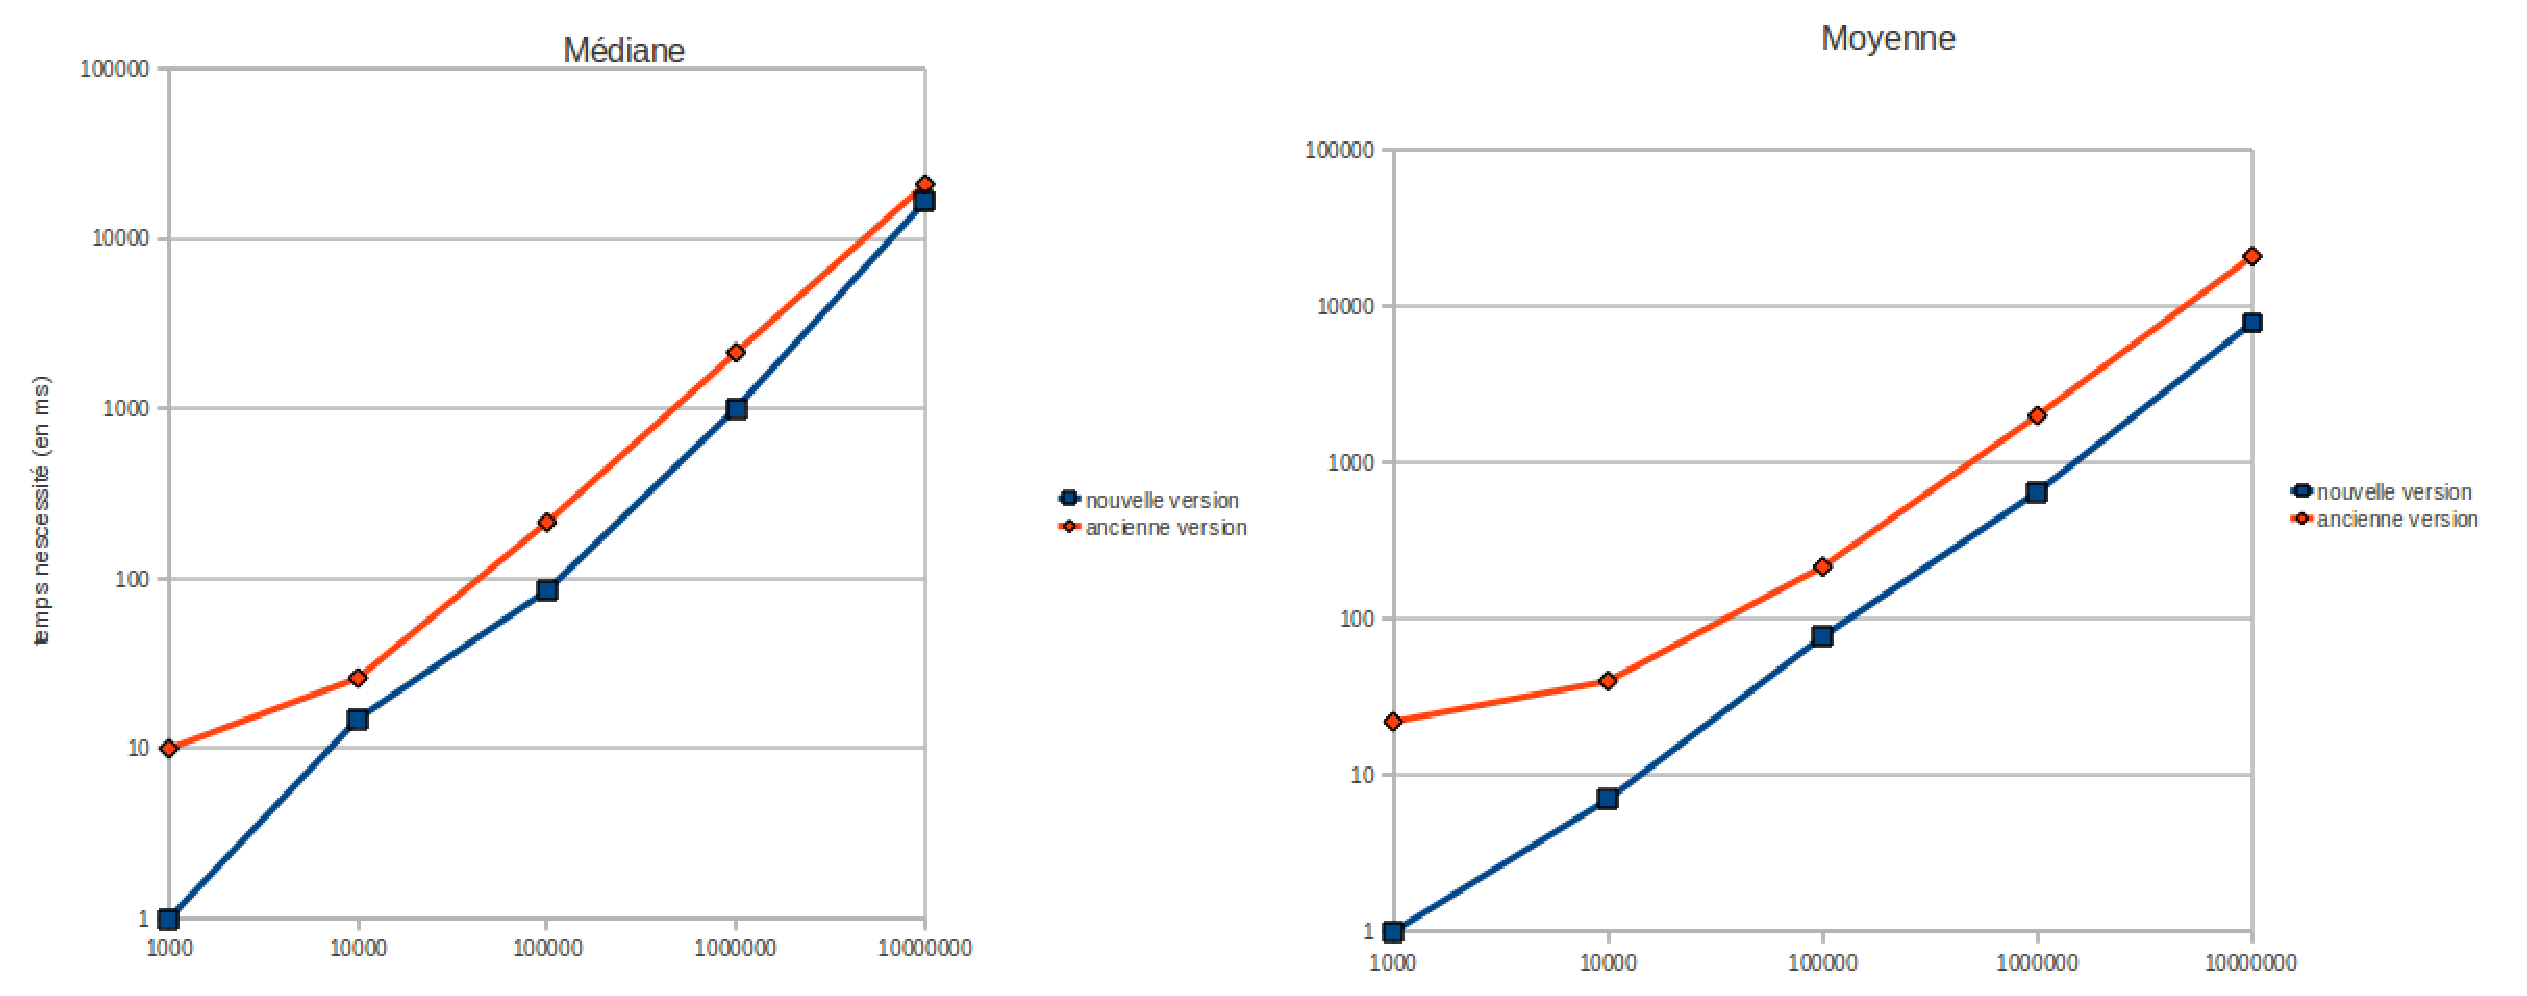
\includegraphics[width=15cm]{MoyenneMediane.eps}
\end{center}
\caption{Performances de M\'ediane et Moyenne}
\label{tab:medmoy}
\end{figure}

Le tableau \ref{tab:numaverage} montre les performances de chacune de ces options (\textbf{og} et \textbf{ng} signifiant respectivement << \textbf{old generation} >> et << \textbf{new generation} >> ) : 
\newline
On observe successivement pour chaque test le temps d'ex\'ecution (en ms) sur en premi\`ere ligne , le nombre d'allocations m\'emoire sur la deuxi\`eme et la m\'emoire
allou\'ee sur la troisi\`eme.
\newline

\begin{table}[h]
\begin{center}
\begin{tabular}{|c|c|c|c|c|c|c|}

\hline
Nb de donn\'ees & moy (og) & moy (ng) & m\'ed (og) & m\'ed (ng) & mod (og) & mod (ng)  \\
\hline
 \multirow{3}*{1000} & 22 & 1 & 10 & 1 & 11 & 2 \\
\cline{2-7}
 & 1693 & 1 & 1693 & 1004 & 1693 & 2003 \\
\cline{2-7}
 & 183ko & 352o & 183ko & 4Mo & 183ko & 6Mo \\
\hline
 \multirow{3}*{10000} & 40 & 7 & 26 & 15 & 40 & 107 \\
\cline{2-7}
 & 1693 & 1 & 1693 & 10000 & 1693 & 2003 \\
\cline{2-7}
 & 183ko & 352o & 183ko & 400Mo & 183ko & 600Mo \\
\hline
100000 & 215 & 77 & 214 & 85 & 279 & 8024 \\
\hline
1000000 & 1991 & 647 & 2133 & 1004 &  &  \\
\hline
10000000 & 20748 & 7799 & 20802 & 12530 &  & \\
\hline
\end{tabular}
\end{center}
\caption{Performances de M\'ediane et Moyenne}
\label{tab:numaverage}
\end{table}
Remarque : faute de temps (l'ex\'ecution de valgrind \'etant tr\`es lente) les tests de m\'emoire n'ont pas \'et\'e fait pour de grandes s\'eries de nombres.
\newline
On peut remarquer que conform\'ement \`a nos attentes les temps d'ex\'ecution des nouveaux programmes sont bien inf\'erieurs \`a ceux des anciens,
 n\'eanmoins certains d'entre-eux ont des consommations de m\'emoire beaucoup plus importantes, cela est d\^u au fait que certains de nos programmes 
ne supportent pas encore les flux de donn\'ees (en particulier la fonction qui calcule le mode), nous en reparlerons dans la partie optimisation.
Le probl\`eme de la gestion des flux de donn\'ees est un probl\`eme r\'ecurrent en algorithmie : certains programmes ont besoin d'un historique 
des donn\'ees pour faire leur calcul, ce qui devient un probl\`eme pour un grand nombre de donn\'ees.

\subsection{Comparaisons de nombres d\'ecimaux}

Dans cette partie la probl\'ematique est quasiment la m\^eme que dans la partie pr\'ec\'edente, \`a l'exception pr\`es qu'ici seulement les fonctions 
numinterval et numnormalize sont sujette au probl\`eme des flots de donn\'ees. Les tests effectu\'ees sur numbound et numround tableau \ref{fig:bouround}
et figure \ref{fig:bouround} sont donn\'es en ms.
\newline

\begin{table}[h]
\begin{center}
\begin{tabular}{|c|c|c|c|c|}
\hline
Nb de donn\'ees & numbound (og) & numbound (ng) & numround (og) & numround (ng) \\
\hline
1000 & 15 & 3 & 49 & 7 \\
\hline
10000 & 30 & 7 & 84 & 18 \\
\hline
100000 & 180 & 67 & 529 & 89 \\
\hline
1000000 & 2003 & 897 & 4152 & 1217 \\
\hline
10000000 & 19005 & 8669 & 42691 & 11842 \\
\hline
\end{tabular}
\caption{Performances de numbound et numround}
\end{center}
\label{tab:numbound}
\end{table}

\begin{figure}[h]
\begin{center}
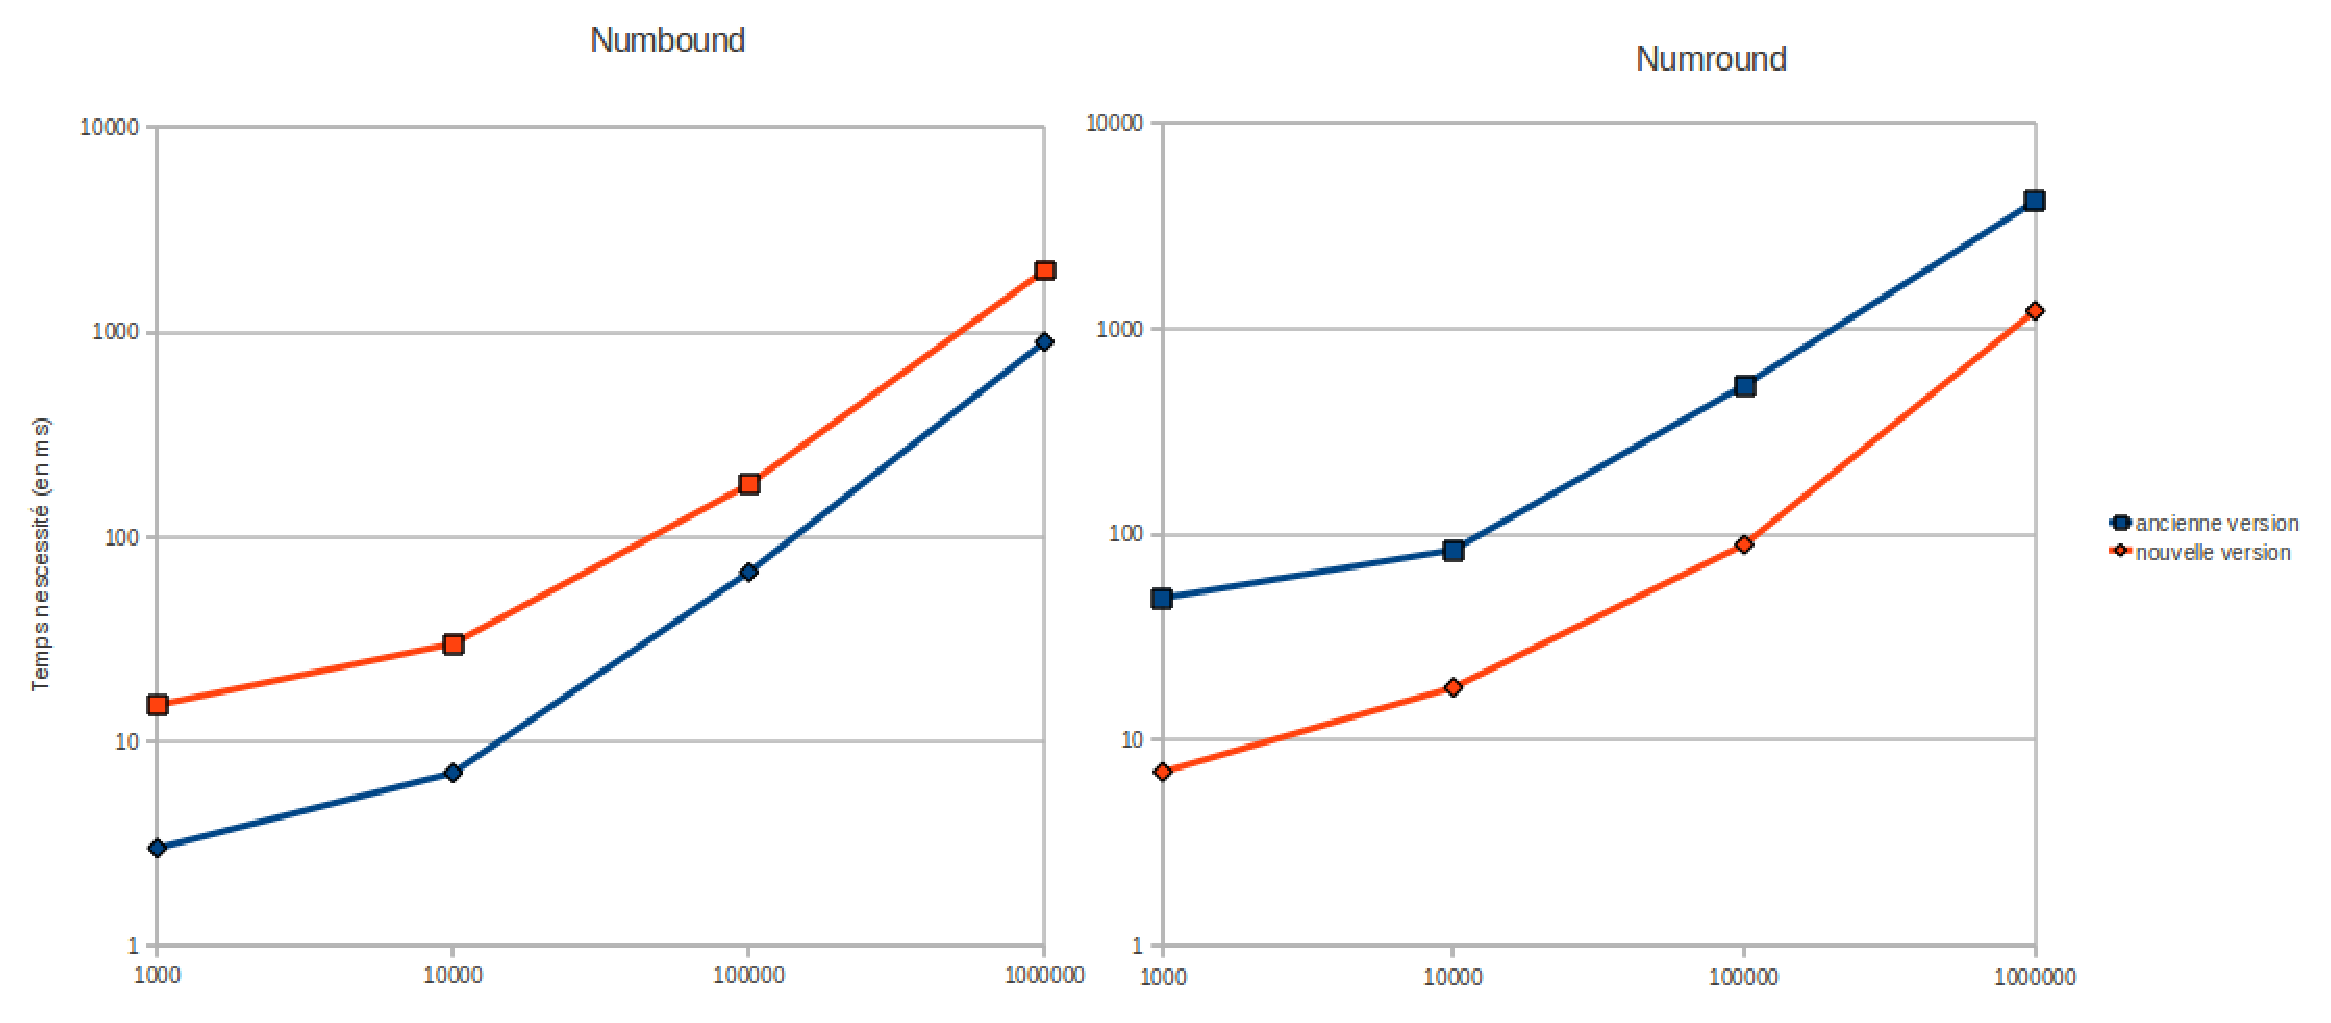
\includegraphics[width=15cm]{NumboundNumround.eps}
\end{center}
\caption{Performances de numbound et numround}
\label{fig:bouround}
\end{figure}

\begin{table}[h]
\begin{center}
\begin{tabular}{|c|c|c|c|c|}
\hline
Nb de donn\'ees & numinterval (og) & numinterval (ng) & numnormalize (og) & numnomrmalize (ng)\\
\hline
 \multirow{2}*{100} & 2075 (fuites) & 101 & 1693 (fuites) & 6 \\
\cline{2-5}
 & 210ko & 40ko & 183ko & 16ko \\
\hline
 \multirow{2}*{1000} & 2075 (fuites) & 1001 & 1693 (fuites) & 12 \\
\cline{2-5}
 & 210ko & 4Mo & 183ko & 262ko \\
\hline
 \multirow{2}*{10000} & 2075 (fuites) & 10000 & 1693 (fuites) & 16 \\
\cline{2-5}
 & 210ko & 400Mo & 183ko & 2Mo \\
\hline
 \multirow{2}*{100000} & 2075 (fuites) & 100000 & 1693 (fuites) & 19 \\
\cline{2-5}
 & 210ko & 40Go & 183ko & 16Mo \\
\hline
\end{tabular}
\caption{Utilisation de la m\'emoire de numinterval et de numnormalize, nombre d'allocations m\'moire et m\'emoire allou\'ee}
\end{center}
\label{tab:numinterval}
\end{table}

\begin{figure}[h]
\begin{center}
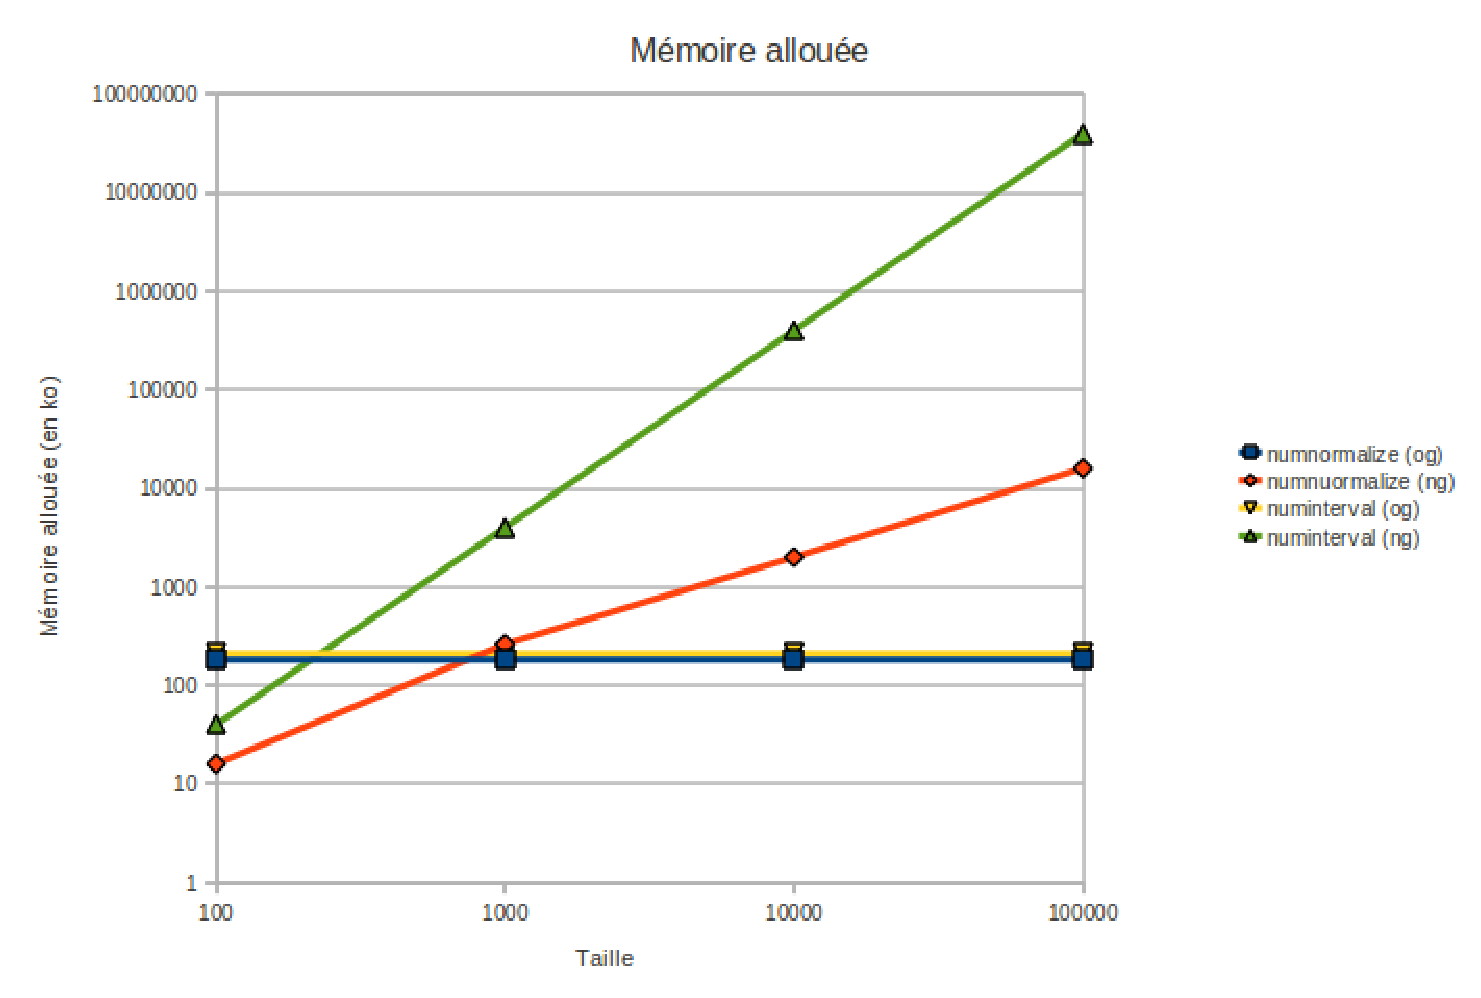
\includegraphics[width=11cm]{Memallouee.eps}
\end{center}
\label{fig:numinterval}
\caption{Utilisation de la m\'emoire pour numinterval et numnormalize}
\end{figure}

Les r\'esultats sont particuli\`erement exceptionels en mati\`ere de temps d'ex\'ecution mais il persiste le probl\`eme de l'utilisation de la
 m\'emoire pour numinterval (figure 4.3 et tableau 4.3).
\newline

\subsection{G\'en\'eration et modifications de nombre d\'ecimaux}

Dans cette partie la probl\`ematique est diff\'erente car aucun de ces programmes n'est destin\'e \`a travailler sur des flux de donn\'ees, 
d'ailleurs numrange et numrandom n'ont m\^eme pas de fichier en argument ils ne servent qu'\`a g\'en\'erer des nombres ou s\'eries de nombres.
C'est pourquoi on effectue diff\'erents tests pour ces fonctions : pour numgrep et numprocess on peut toujours regarder leur comportement selon la taille du fichier d'entr\'ee.
Tandis que pour numrange on peut faire augmenter la taille du fichier \`a g\'en\'erer et pour numrandom la taille de l'intervalle dans lequel on prend le chiffre (figure \ref{fig:randomrange}).
Pour numprocess nous avons fait les tests pour plusieurs op\'erations et expressions seules certaines ont \'et\'e retenues pour le rapport. 
Les tableaux de performances se trouvent en annexe.


\begin{figure}[h]
\begin{center}
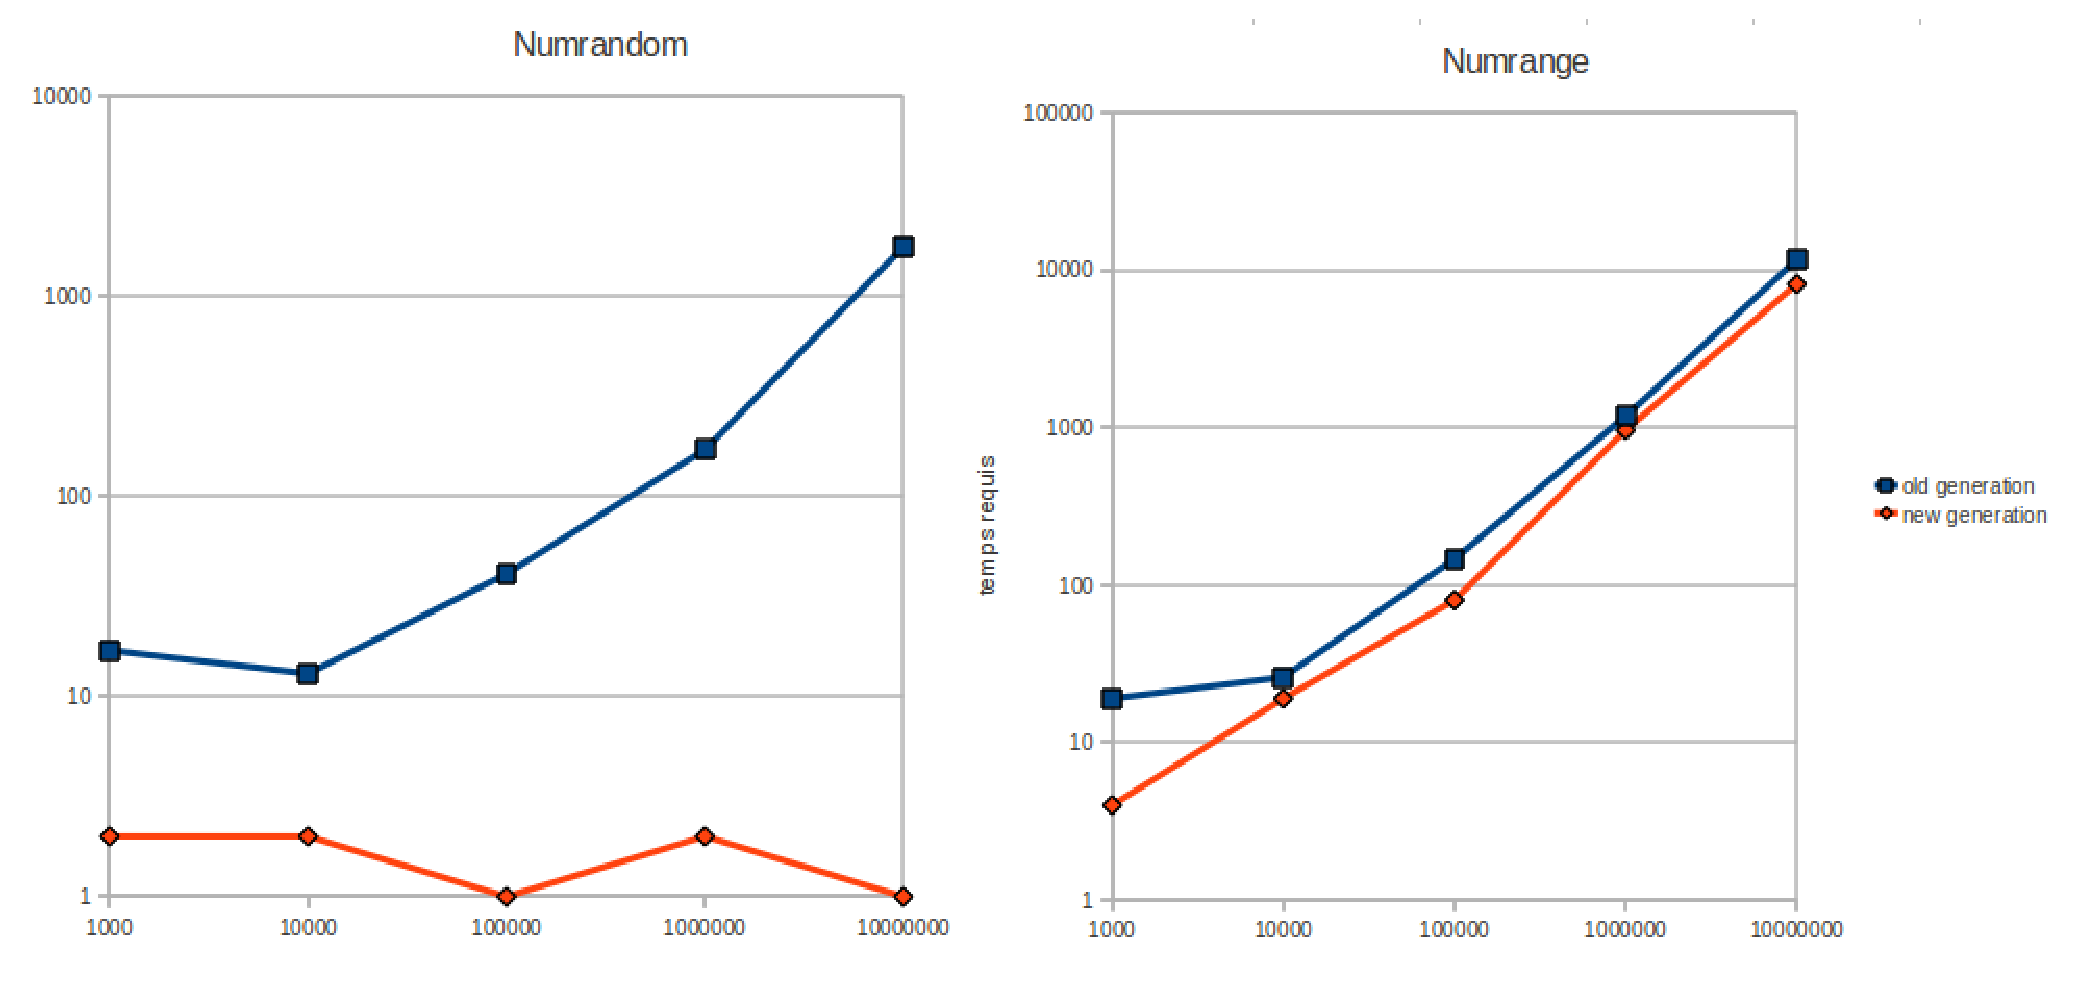
\includegraphics[width=15cm]{randomrange.eps}
\end{center}
\caption{Performances de numrandom et numrange}
\label{fig:randomrange}
\end{figure}

\begin{figure}[h]
\begin{center}
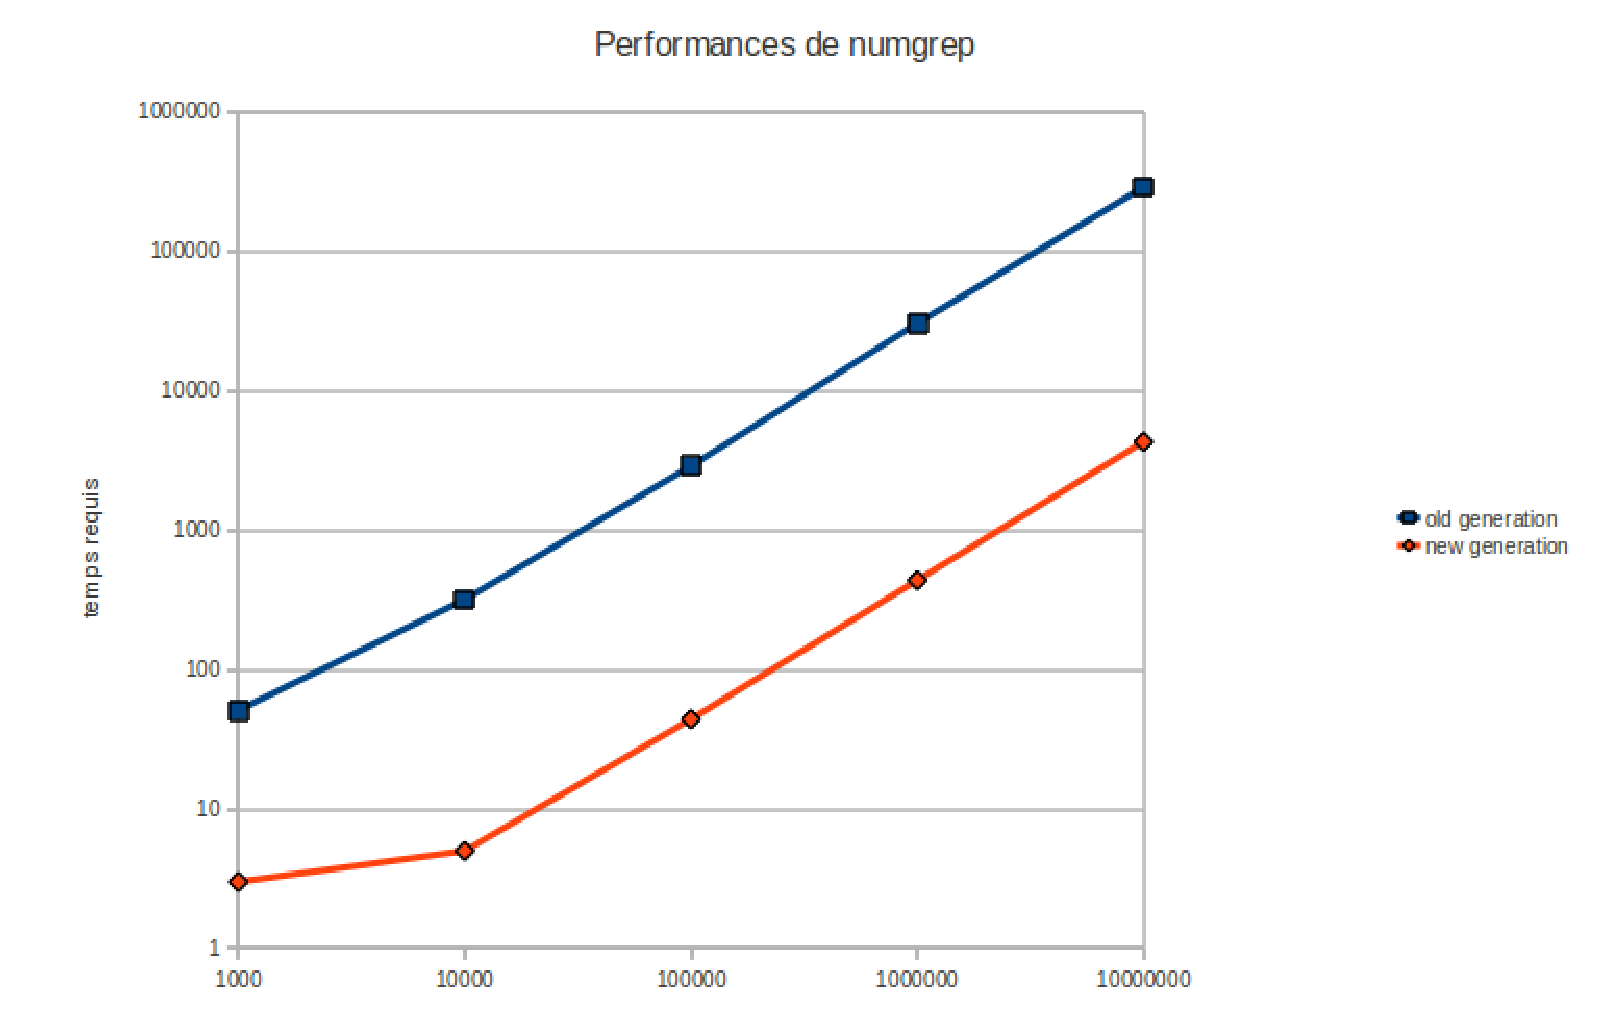
\includegraphics[width=9cm]{numgrep.eps}
\end{center}
\caption{Performances de numgrep}
\label{fig:numgrep}
\end{figure}


\begin{figure}[h]
\begin{center}
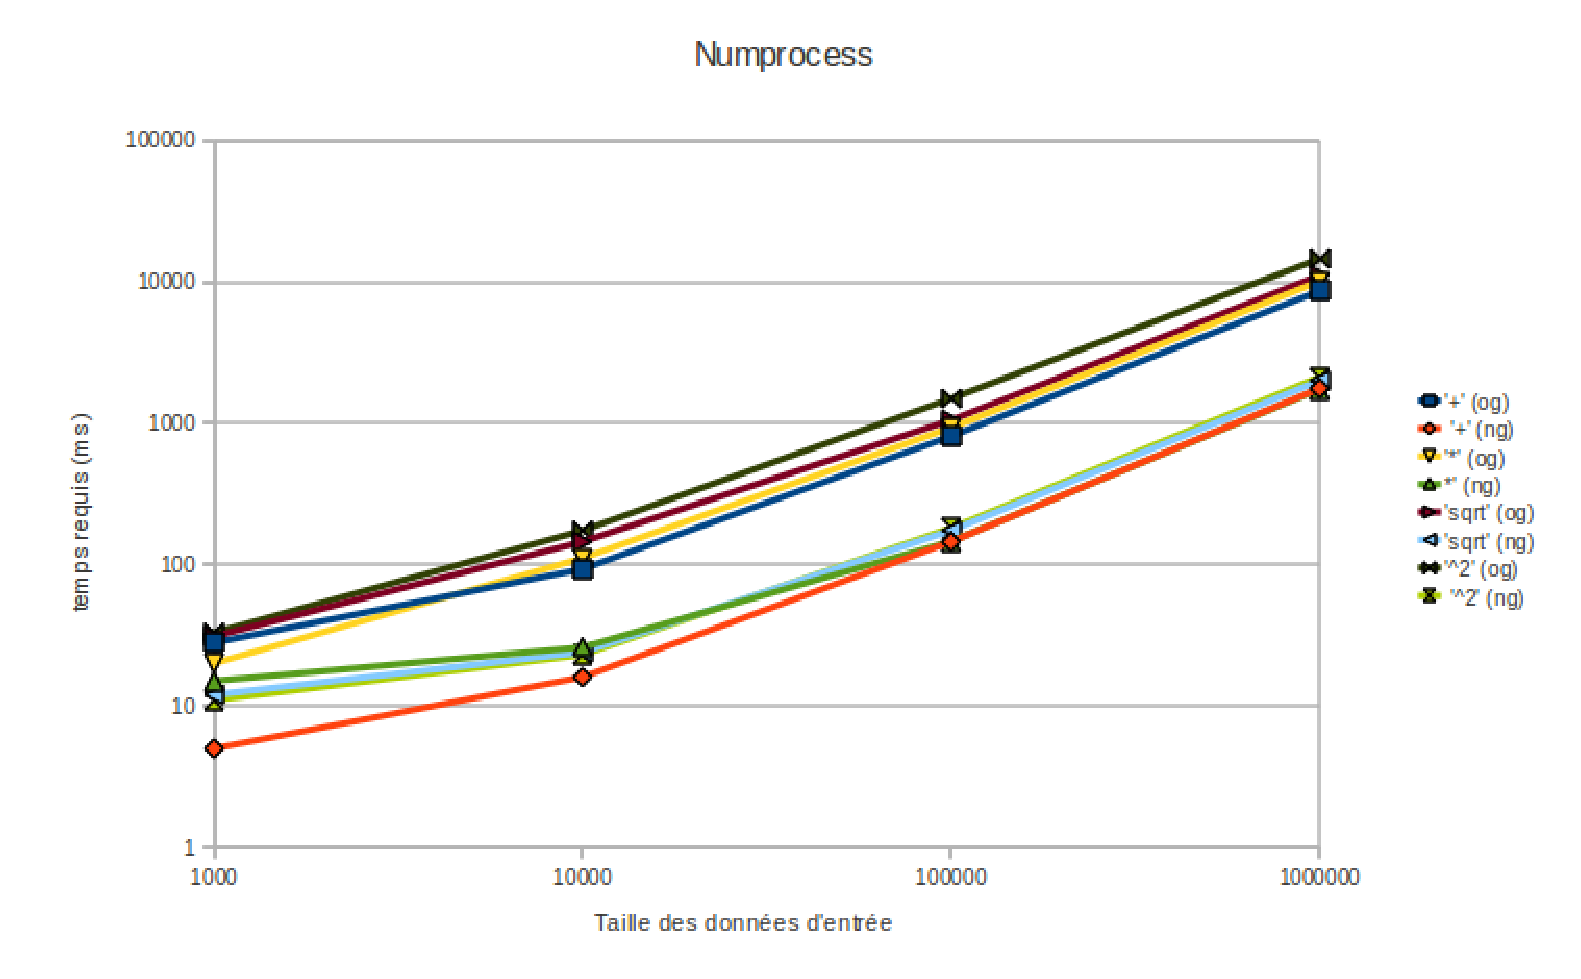
\includegraphics[width=9cm]{numprocess.eps}
\end{center}
\caption{Performances de certaines op\'erations de numprocess}
\label{fig:numprocess}
\end{figure}

Les r\'esultats en terme de temps pour numgrep (figure \ref{fig:numgrep}) et numprocess (figure \ref{fig:numprocess}) sont plut\^ot bons, il ny a quasiment pas d'utilisation de la m\'emoire dans numprocess et numrange contrairement aux anciennes versions. 
Nous avions aussi fait des tests en changeant le nombre d'intervalles dans les expressions et on peut voir que la progression est lin\'eaire, les programmes se comportent donc bien s'il y a beaucoup d'intervalles.

On peut ajouter que les programmes de l'ancienne biblioth\`eque comportent tous des fuites de m\'emoires (memory leaks) qui ne sont plus pr\'esent 
dans notre biblioth\`eque.

\section{Optimisations}

Nous avons vu les probl\`emes li\'es \`a la gestion des flux, il y a diff\'erents moyens pour pallier \`a ce probl\`eme.
C'est ce que nous allons voir dans cette partie.

Il y a trois types d'optimisation majeure que nous avons utilis\'e :

La r\'eduction du nombre d'allocation qui peut se r\'ev\'eler \^etre faramineux quand on fait des tests sur de grands nombres de donn\'ees \'etait notre priorit\'e.
Pour ce faire, nous avons multipli\'e la taille des allocations par deux \`a chaque allocation ainsi nous avons divis\'e le nombre d'allocations par une puissance de deux.
Par exemple une ex\'ectution d'un programme n\'ecessitant 1024 allocations n'a besoins plus que de 11 allocations. Bien s\^ur la taille des allocations est tr\`es sup\'erieure mais le nombre d'op\'erations d'allocation qui est chronophage a \'et\'e grandement r\'eduit :
On r\'eduit le temps d'ex\'ecution mais pas la m\'emoire allou\'ee qui peut d'ailleur \^etre augment\'ee.

La modification d'algorithmes, par exemple dans numround, permet un code plus lisible et facile \`a comprendre mais n'am\'eliore pas les performances car nous nous en sommes tenu aux premiers algorithmes trouv\'es pour les calculs des r\'esultats.
Les programmes sont maintenant \`a l'\'epreuve des utilisateurs non avertis : par exemple une faute de frappe n'entra\^inera pas une boucle infinie mais un message d'erreur appropri\'e sera affich\'e.

Enfin, l'utilisation de fichiers temporaires pas forc\'ement n\'ecessaires a \'et\'e bannie : le r\'esultat est peut-\^etre moins joli mais les performances sont grandement am\'elior\'ee.

Afin de donner un exemple de ces am\'eliorations, voici les r\'esultats obtenus sur la fonction numaverage : 
En bleu la version initiale, en rouge la premi\`ere version que nous avons faite et en jaune la version optimis\'ee.
Comme pour les graphes p\'ec\'edents, on peut observer le nombre de donn\'ees en abscisse et le temps requis en ordonn\'ee.

\begin{figure}[h]
\begin{center}
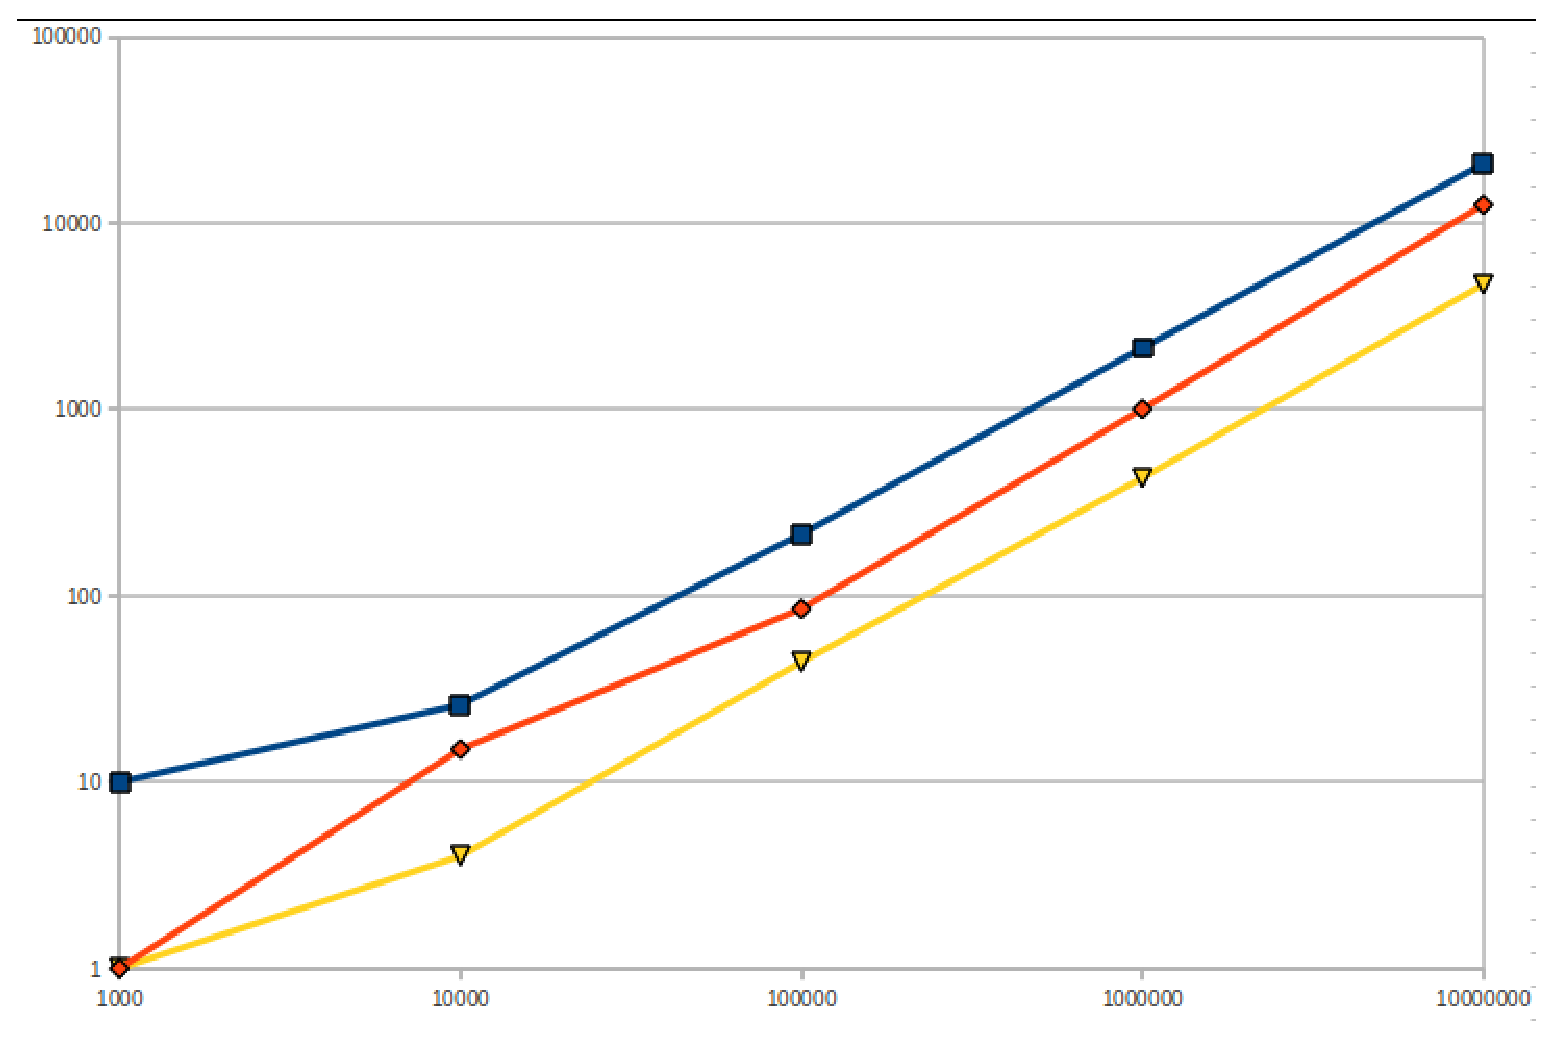
\includegraphics[width=9cm]{median.eps}
\end{center}
\caption{Comparaison des performances des versions de l'option ``M\'ediane'' de numaverage}
\label{fig:numprocess}
\end{figure}
 % chapitre 4

%\addcontentsline{toc}{chapter}{Conclusion}
\chapter*{Conclusion}

Au cours de notre projet, nous avons appris \`a suivre une d\'emarche de conception sp\'ecifique en vue d'aboutir \`a la cr\'eation
puis \`a la publication d'un paquet Debian. Notre travail se basait sur une biblioth\`eque de calcul num\'erique existante et d\'ej\`a
distribu\'ee num-utils. Nous avons pu montrer notre capacit\'e \`a analyser un code \'ecrit par un autre d\'eveloppeur, puis \`a l'optimiser dans 
un autre langage, en C, pr\'esentant des avantages mais \'egalement des inconv\'enients. Nous avons appris, progressivement, \`a utiliser des outils
de d\'eveloppement : le gestionnaire de version, la cr\'eation de pages de manuel (man pages), les autotools puis les outils de cr\'eation de paquets Debian. Finalement, nous obtenons une premi\`ere
version de la biblioth\`eque num-utils-ng.
\newline
\newline
Maintenant, nous devons continuer \`a am\'eliorer notre biblioth\`eque num\'erique. Il nous faut ajouter de nouvelles fonctionnalit\'es utiles et \'egalement 
corriger les bugs qui subsistent encore dans la premi\`ere version de notre biblioth\`eque num\'erique. Il nous faut aussi optimiser certains des 
algorithmes impl\'ement\'es, qui quelquefois sont un plus lents ou utilisent plus de m\'emoire que la version d\'ej\`a publi\'ee. Enfin il nous restera \`a
diffuser notre paquet. Nous avons cr\'e\'e un site internet (en construction actuellement) pour nous permettre de proposer notre distribution open source,
d'offrir une assistance technique aux futurs utilisateurs et de r\'epondre \`a leurs suggestions
\newline
\newline
L'objectif final \'etant ainsi la publication, dans les vraies archives Debian, du paquet num-utils-ng.

%\markboth{Conclusion}{Conclusion}


\newpage\cleardoublepage

\bibliographystyle{unsrt}\bibliography{bib/references}
\addcontentsline{toc}{chapter}{R\'ef\'erences}

\newpage\cleardoublepage\addcontentsline{toc}{chapter}{Glossaire}
\chapter*{Glossaire}
\begin{description}

\item[Allocation] : l'alloction est l'op�ration qui consiste � r�server de la place dans la m�moire, c'est une op�ration qui demande un peu de ressources et qui est donc � utiliser le moins possible.
\item[autotools] : outils fournis par le projet GNU pour faciliter la fabrication de paquets � partir du code source d'un programme.
\item[Distribution] : Une distribution de GNU/Linux est une version d'un syst�me d'exploitation, il y en a plusieurs car il y a plusieurs syst�mes d'exploitation utilisant le m�me noyau : Ubuntu, Debian, Red Hat.
\item[Flux ou Flot de donn�es] : le flot de donn�es est la succession de donn�es d'un certain type, qui peuvent se poursuivre pendant un temps ind�fini.
\item [fuite de m�moire] : occupation croissante et non contr�l�e ou non d�sir�e de la m�moire d'un ordinateur. 
\item[Gestionnaire de version] : logiciel qui permet de stocker un ensemble de fichiers en conservant la chronologie de toutes les modifications qui ont �t� effectu�es dessus.
\item[Langage compil�] : langage dans lequel le code est traduit en langage binaire pour une compr�hension direct du processeur. Un programme �crit en langage compil� est traduit en instructions lisibles par la machine et peut �tre ex�cut� ind�pendamment de tout autre programme.
\item[Langage interpr�t�] : langage dans lequel le code n'est pas compil� . Un programme �crit en langage interpr�t� n'est pas ex�cut� directement par la machine mais par un autre programme.
\item[logiciel open source] : logiciel dont l'utilisation, l'�tude, la modification et la duplication en vue de sa diffusion sont permises, techniquement et l�galement.
\item[Makefile] : un Makefile est un fichier utilis� par la commande make des distributions GNU/Linux permettant l'automatisation de t�ches simples telles que la compilation.
\item[mode] : le mode d'une s�rie de nombres est le nombre qui apparait le plus de fois dans la s�rie.
\item[Paquet] : un paquet Debian est un paquet rassemblant les sources d'un programme et comment les installer, ainsi que les d�pendances n�cessaires. On les trouve typiquement dans les archives Debian et elle servent � installer des programmes facilement sous Ubuntu ou Debian.

\end{description}

\markboth{Glossaire}{Glossaire}

\appendix
\chapter{Planification du projet}

\section{Planning du projet}

Nous avons \'etabli le planning de la figure \ref{fig:planning} pour notre projet. Les barres gris\'ees correspondent \`a la plannification initiale, les barres bleues au 
planning r\'eel.
\newline
Notre travail s'est effectu\'e en trois \'etapes. Premi\`erement, l'analyse du besoin et la r\'edaction du cahier des charges fonctionnel.
Deuxi\`emement, la phase de conception, de r\'ealisation et de test de notre solution, estim\'ee \`a 64 jours.
Enfin, la phase de conception du rapport et du poster.
Comme notre biblioth\`eque est constitu\'ee de dix utilitaires, nous les avons r\'eparti entre nous trois. Ainsi, nous avons chacun effectu\'e les diff\'erentes
\'etapes de la phase de d\'eveloppement. C'est pourquoi, aucun nom n'est associ\'e \`a une t\^ache en particulier.

\section{Analyse des \'ecarts}

La phase de codage a dur\'e deux mois au lieu de six semaines. Cela s'explique par les nombreuses am\'eliorations apport\'ees au code au fur et \`a mesure.
Nous avons rattrap\'e ce retard en effectuant la cr\'eation des fichiers binaires en une semaine au lieu de deux semaines.	 
Nous avons commenc\'e la r\'edaction du rapport plus tard afin de finir le plus rapidement possible la phase de d\'eveloppement.
Nous avions \'egalement pr\'evu deux semaines pour cr\'eer le poster mais nous avons pu le finir en une semaine.
\newline
Dans la partie << Suivi du projet >>, vous pouvez constater que nous n'avons pas pu effectuer toute les r\'eunions pr\'evues. A cause de l'indisponibilit\'e de notre
tuteur lors de conf\'erences, nous avons d\^u d\'ecaler nos r\'eunions. Toutefois, nous avons pu communiquer facilement \`a distance.
On constate donc que nous avons globalement suivi la plannification initiale.

\newpage
\begin{figure}[h]
\begin{minipage}[c]{0mm}
\includegraphics[width=15cm,height=21cm]{planning.eps}
\end{minipage}
\caption{Planning du projet}
\label{fig:planning}
\end{figure}


\chapter{Cahier des charges fonctionnel}

\section{Cahier des charges fonctionnel initial}
Les d\'eveloppeurs effectuent r\'eguli\`erement des calculs sur des flux de donn\'ees, ils ont besoins d'utilitaires simples et performants.
Notre but principal est d'offrir une alternative \`a la biblioth\`eque num-utils qui propose des utilitaires de calcul num\'erique. 
Cette biblioth\`eque est impl\'ement\'ee en Perl, l'adaptation en C devrait nous permettre d'obtenir de meilleures performances.
Voici le diagramme b\^ete \`a corne qui pr\'esente de fa\c con tr\`es g\'en\'erale le programme que nous devons livrer : 

\begin{figure}[h]
\begin{center}
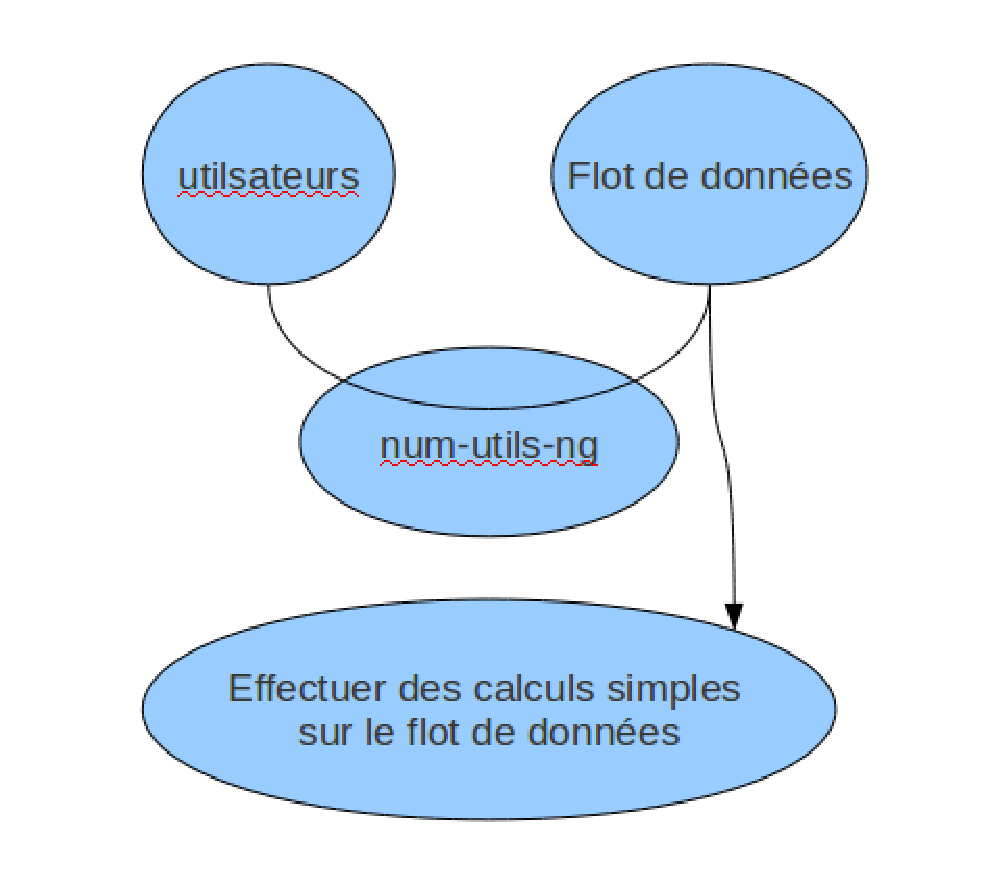
\includegraphics[width=9cm]{beteacorne.eps}
\end{center}
\caption{Diagramme B\^ete \`a cornes}
\label{fig:numprocess}
\end{figure}

Nous avons distingu\'e plusieurs fonctions contraintes pour notre biblioth\`eque : 
\newline
FP1 : Pouvoir effectuer des calculs simples sur des flots de donn\'ees.
\newline

FC1 : Les utilitaires propos\'es doivent \^etre plus rapide que les anciens.
\newline
FC2 : La biblioth\`eque doit \^etre pr\^ete sous un certain d\'elai.
\newline
FC3 : Cette biblioth\`eque doit \^etre \'ecrite dans un certain langage.
\newline
FC4 : Les programmes doivent \^etre libre.
\newline
FC5 : Les utilisateurs doivent pouvoir se servir facilement de ces utilitaires.
\newline
FC6 : La biblioth\`eque finale devra \^etre accessible  \`a tous.
\newline
FC7 : Il ne doit pas y avoir de bogues.
\newline


Les fonctions contraintes sont expos\'ees plus pr\'ecis\'ement dans le tableau fonctionnel ci-dessous.

\begin{table}[h]
\begin{center}
\begin{tabular}{|c|c|c|c|}
\hline
 & Crit\`ere & Niveau & Flexibilit\'e \\
\hline
 FC1 & Rapidit\'e & 10 fois plus rapide & 2 \\
\hline
 FC2 & D\'elai & 5 mois & 0 \\
\hline
 FC3 & Langage & C & 1 \\
\hline
 FC4 & Licence & GNU General Public License & 0 \\
\hline
 FC5 & Facilit\'e d'utilisation & M\^eme commandes qu'avant & 2 \\
\hline
 FC6 & Accessibilit\'e & Disponible sur le d\'ep\^ot officiel Debian & 1 \\
\hline
 FC7 & Nombre de bogues & 0 & 1 \\
\hline
\end{tabular}
\caption{Tableau Fonctionnel}
\end{center}
\label{tab:tabfonctionnel}
\end{table}

Flexibilit\'e : \newline
0 = imp\'eratif\newline
1 = peu n\'egociable\newline
2 = n\'egociable\newline
3 = tr\`es n\'egociable\newline

\section{Comparaison avec la version finale}
Nous voici \`a la fin de notre projet et d'une mani\`ere g\'en\'erale nous avons aboutit \`a une version op\'erationnelle de la biblioth\`eque mais nous 
allons maintenant voir si elle est conforme au cahier des charge que nous avions r\'edig\'e.

La fonction principale est bien entendu v\'erifi\'ee puisque nos utilitaires fonctionnent tous.

Prenons les fonctions contraintes une \`a une afin de v\'erifier si elles sont respect\'ees :

\begin{itemize}
\item [\textbullet] \textbf{FC1 : Les utilitaires propos\'es doivent \^etre plus rapides que les anciens.}
\newline
\normalsize
Nous avions esp\'er\'e aboutir \`a des programmes dix fois plus rapides que ceux de la version ant\'erieure mais cela n'a pas \'et\'e le cas : 
en moyenne nous atteignons des temps d'ex\'ecutions trois fois moins \'elev\'es. N\'eanmoins cette condition est n\'egociable et ne discr\'edite pas notre solution.
\item [\textbullet] \textbf{FC2 : La biblioth\`eque doit \^etre pr\^ete sous un certain d\'elai.}
\newline
\normalsize
Le d\'elai impos\'e de cinq mois a bien \'et\'e respect\'e.
\item [\textbullet] \textbf{FC3 : Cette biblioth\`eque doit \^etre \'ecrite dans un certain langage.}
\newline
\normalsize
Le langage C a bien \'et\'e utilis\'e et nous a permis un grand gain de vitesse.
\item [\textbullet] \textbf{FC4 : Les programmes doivent \^etre libre.}
\newline
\normalsize
La licence sous laquelle est diffus\'ee notre biblioth\`eque est GNU General Public License, ce crit\`ere est donc respect\'e.
\item [\textbullet] \textbf{FC5 : Les utilisateurs doivent pouvoir se servir facilement de ces utilitaires.}
\newline
\normalsize
Les commandes et options utilis\'ees sont exactement les m\^emes que dans la version ant\'erieure à l'exception des ``..'' remplac\'es par les `` : '' dans les expressions pour numrange et numrandom.
\item [\textbullet] \textbf{FC6 : La biblioth\`eque finale devra \^etre accessible  \`a tous.}
\newline
\normalsize
Le biblioth\`eque est disponible sur le d\'ep\^ot officiel Debian.
\item [\textbullet] \textbf{FC7 : Il ne doit pas y avoir de bogues.}
\newline
\normalsize
Il reste quelques bogues mineurs dont pour lesquels nous n'avons pas trouv\'es de solutions, ils r\'esultent pour la plupart d'un mauvaise utilisation des utilitaires propos\'es.
\end{itemize}

En conclusion on peut voir que la version finale de la biblioth\`eque est conforme au cahier des charges fonctionnels, notre solution est donc viable.

\chapter{Analyse personnelle du projet}

\begin{itemize}
\item [\textbullet] \Large \textbf{Reuven Benichou}
\newline
\normalsize
\item [\textbullet] \Large \textbf{Edern Hotte}
\newline
\normalsize
J'ai trouv\'e ce projet tr\`es int\'eressant. Je dois avouer qu'au d\'epart, j'avais des appr\'ehensions quant \`a la quantit\'e de code que nous avions \`a livrer qui s'est finalement 
r\'ev\'eler ne pas \^etre si \'enorme que \c ca. J'ai appris beaucoup de choses : les \'etapes de la publication d'un paquet Debian, l'\'elaboration et l'\'ecriture de scripts de tests 
en bash et comment s'assurer qu'un programme s'ex\'ecutera comme pr\'evu m\^eme si l'utilisateur ne l'utilise pas de fa\c con normale. J'ai d\'ecouvert des outils tr\`es utiles au d\'eveloppement,par exemple Valgrind qui permet de retrouver
d'o\`u proviennent certaines erreurs de segmentations et de contr\^oler les fuites de m\'emoire. J'ai aussi appris \`a utiliser les Makefile permettent un tr\`es grand gain
de temps grace \`a l'automatisation de certaines taches comme la compilation des sources ou la suppression des fichiers interm\'ediaires. Certaines fonctions du C m'\'etaient m\'econnues avant ce projet,
getopt, qsort ou encore perror sont de nouveaux mots dans mon vocabulaire. Notre encadrant nous a bien aid\'e en nous suivant et nous conseillant tout au long du d\'eveloppement et l'ambiance du groupe \'etait plut\^ot bonne.\newline
\item [\textbullet] \Large \textbf{Flavien Moullec}
\newline
\normalsize
Ce projet a \'et\'e pour moi int\'eressant et instructif. Au d\'ebut, je ne savais pas exactement quel type de travail nous aurions \`a effectuer.
Comme notre travail \'etait de suivre les \'etapes amenant \`a la cr\'eation d'un paquet Debian, je ne connaissais pas les outils de
d\'eveloppement que nous avons utilis\'e. Ce projet m'a permis de cr\'eer le planning du projet et de me rendre compte de la difficult\'e d'en r\'ealiser un
et de le respecter ensuite. Je suis assez content d'avoir appris \`a utiliser des outils de d\'eveloppement comme les autotools ou le programme de cr\'eation de 
paquet Debian, que j'ai trouv\'e assez int\'eressant.

J'ai trouv\'e certaines parties du projet, notamment les script de tests assez difficiles \`a comprendre, ou dans l'utilisation de commandes Unix qui pouvaient
simplifier notre code quelquefois, si nous les avions connues au d\'ebut.

Notre encadrant nous a bien suivi, en nous donnant des conseils techniques et disponible pour r\'epondre \`a nos questions.
Je suis content de mon groupe car nous \'etions dans l'ensemble plut\^ot motiv\'e pour faire avancer le projet.


\end{itemize}

\chapter{R\'epartition de la r\'edaction et de la relecture du rapport}

Voici la r\'epartition de l'\'ecriture et de la relecture du rapport :
\newline
\section{\'Ecriture}
\begin{itemize}
  \item[-] R\'esum\'e/Abstract : Edern
  \item[-] Chapitre 1 : \textbf{Introduction} : Reuven
  \item[-] Chapitre 2 : \textbf{La Biblioth\`eque num-utils} : Flavien
  \item[-] Chapitre 3 : \textbf{D\'emarche de conception effectu\'e}, section 1 : Reuven
  \item[-] Chapitre 3 : \textbf{D\'emarche de conception effectu\'e}, section 2 et 3 : Flavien
  \item[-] Chapitre 4 : \textbf{Tests et Optimisation} : Edern
  \item[-] Conclusion : Flavien
\newline
\end{itemize}
\section{Relecture}
\begin{itemize}
  \item[-] R\'esum\'e/Abstract : Reuven
  \item[-] Chapitre 1 : \textbf{Introduction} : Flavien
  \item[-] Chapitre 2 : \textbf{La Biblioth\`eque num-utils} : Edern
  \item[-] Chapitre 3 : \textbf{D\'emarche de conception effectu\'e} : Edern
  \item[-] Chapitre 4 : \textbf{Tests et Optimisation} : Flavien
  \item[-] Conclusion : Edern
\end{itemize}


\newpage
\cleardoublepage
\addcontentsline{toc}{chapter}{Index}
\markboth{Index}{Index}
\printindex

\newpage\thispagestyle{empty}   % affiche la dernière page du rapport
\vspace*{55mm}
\hspace{48mm}
\begin{minipage}[c]{0mm}
  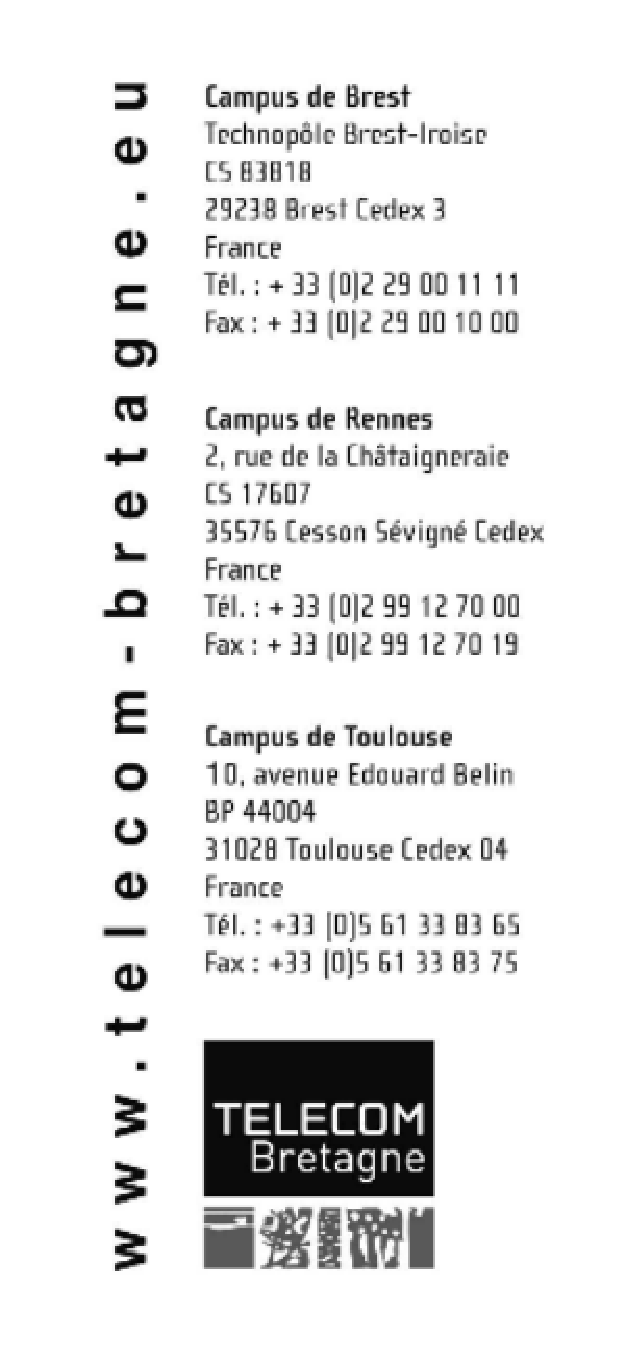
\includegraphics[width=55mm]{lastPage.eps}
\end{minipage}

\end{document}
